\documentclass[border=3pt,tikz]{standalone}
\usepackage{amsmath}
\usetikzlibrary{calc}
\usetikzlibrary{arrows.meta} % for arrow size
\begin{document}
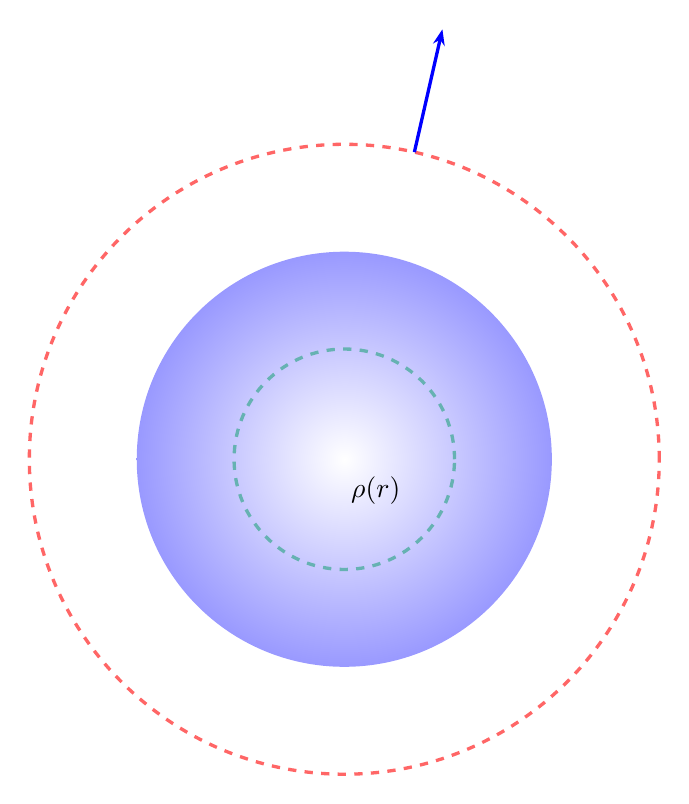
\begin{tikzpicture}[scale=2]
    \coordinate (P1) at (0.445, 1.950);
    \node[circle,outer color=blue!40!white,inner color=white,minimum width=150] (radial) at (0,0) {};
    %\draw[-{Stealth[length=2mm]}](0, 0) -- (2, 0) node[above left] {$x$};
    %\draw[-{Stealth[length=2mm]}](0, 0) -- (0, 2) node[below left] {$y$};
    \node at (0.2, -0.2) {$\rho(r)$};
    \draw[color=red!60, dashed, very thick](0,0) circle (2);
    \draw[color=teal!60, dashed, very thick](0,0) circle (0.7);
    \
    \draw[very thick, blue, -{Stealth[length=2mm]}] (P1) -- ($1.4*(P1)$);
    
   \end{tikzpicture}
\end{document}